% !TEX TS-program = xelatex
% !TEX encoding = UTF-8

% This is a simple template for a XeLaTeX document using the "article" class,
% with the fontspec package to easily select fonts.

\documentclass[11pt]{report} % use larger type; default would be 10pt
\usepackage{fontspec} % Font selection for XeLaTeX; see fontspec.pdf for documentation
\defaultfontfeatures{Mapping=tex-text} % to support TeX conventions like ``---''
\usepackage{xunicode} % Unicode support for LaTeX character names (accents, European chars, etc)
\usepackage{xltxtra} % Extra customizations for XeLaTeX
% \fontspec{"[DroidSerif.ttf]"}
% \setmainfont{Droid Serif} % set the main body font (\textrm), assumes Charis SIL is installed
%\setsansfont{Deja Vu Sans}
%\setmonofont{Deja Vu Mono}
\usepackage{amsmath}
\usepackage{xfrac,unicode-math}
\usepackage{siunitx}
\setmathfont[version=cambria]{Cambria Math}
\mathversion{cambria}
\usepackage{cleveref}
% other LaTeX packages.....
\usepackage{geometry} % See geometry.pdf to learn the layout options. There are lots.
\geometry{letterpaper} % or letterpaper (US) or a5paper or....
%\usepackage[parfill]{parskip} % Activate to begin paragraphs with an empty line rather than an indent

\usepackage{graphicx} % support the \includegraphics command and options


\newcommand{\lit}{Li$_2$TiO$_3$}
\newcommand{\lis}{Li$_4$SiO$_4$}
\newcommand{\lio}{Li$_2$O}
\newcommand{\liz}{Li$_2$ZrO$_3$}
\newcommand{\lial}{LiAlO$_2$}
\newcommand{\lisev}{$^7\mathrm{Li}$}
\newcommand{\lisix}{$^6\mathrm{Li}$}
\sisetup{locale = US}



\title{237D Fusion Technology \\
Introduction to Solid Breeder}
\author{Jon Van Lew}
%\date{} % Activate to display a given date or no date (if empty),
         % otherwise the current date is printed 


\begin{document}
\maketitle
\chapter{Lithium Ceramics}
Lithium appears to be the only material suitable for generating tritium for a self-sustained fuel cycle in a commercial fusion reactor. Only a few types of lithium-bearing materials appear to be most promising for tritium breeding. Aside from liquid lithiums (covered in separate lectures in this course), these include solids such as inter-metallic compounds (\textit{e.g.} Li$_7$Pb$_2$), lithium oxide (\lio), and ternary oxides (\textit{e.g.} \lis, \lit, \lial, \liz, \textit{etc.}).








\section{Solid Breeder Material Choices}
For each candidate breeder, a number of performance requirements can be used to measure the relative merits of each material, namely:
\begin{enumerate}
\item Neutronics
\item Thermochemical Properties
\item Physical Properties
\item Tritium Release
\item Compatibility
\item Radiation Effects
\item Fabrication
\end{enumerate}
Operating temperature limits for solid breeders dictate minimum and maximum temperatures for the solids. Simulations performed on many candidate materials indicate that inter-metallic compounds have unacceptable operating temperatures (exceedingly narrow temperature windows) and are unattractive for in-situ tritium recovery. In addition, the compounds of Li$_7$Pb$_2$ and Li$_62$Pb$_38$ were shown to violently react with water and do not offer significant safety advantages compared to liquid breeders (for more, see Clemmer, R. (1980). The Development of Tritium Breeding Blankets for DT-Burning Fusion Reactors. In Fourth ANS Topical Meeting on the Technology of Controlled Nuclear Fusion.).

Thus lithium-based oxides (including ceramic oxides) have become recognized as the most promising tritium-breeding materials for fusion reactor blankets. The lithium-based oxides all, to a certain degree, have desirable characteristics of 
\begin{itemize}
\item{high Li density}
\item{high melting temperature}
\item good tritium release (sufficiently high T release rates and open porosity for purging T)
\item good thermophysical and thermomechanical characteristics
\item ability to withstand the rigors of long-term irradiation at high temperature and under large temperature gradients
\item{desirable neutronics and irradiation characteristics (no bad transmutation nuclides)}
\item{chemical stability \& compatibility with structural material at operating temperatures (in particular thermal stability and chemical inertness are attractive from a safety point of view)}
\end{itemize}



\subsection{Neutronics of lithium}
Natural lithium occurs with the isotopic abundances of 92.58\% for \lisev~and 7.42\% for \lisix~. At low neutron energies, the major tritium and heat producing neutron reaction in lithium ceramics is associated with the \lisix~isotope:
\begin{align}
\mathrm{n} + ~^6\mathrm{Li} &\xrightarrow ~ \alpha + \mathrm{T} +4.78~\text{MeV} \label{eq:Li6T}
\end{align}
The cross-section for this reaction is given in \Cref{fig:xsects}. \lisix~has a very high neutron capture cross-section (3,000 barns) for thermal neutrons $E \approx 10^{-1}$ to $10^{-2}$ eV.

\begin{figure}
\centering
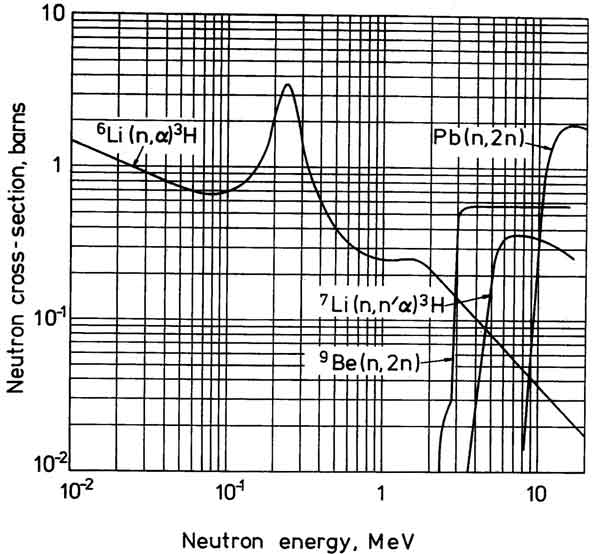
\includegraphics[width=0.8\textwidth]{../images/breeding_xsecs} 
\caption{Cross-sections of various blanket materials. Note the threshold for the \lisev~and neutron multiplying reactions.}
\label{fig:xsects}
\end{figure}

At high neutron energies (14 MeV) found near the first wall of a fusion reactor, the neutron cross section of \lisix~drops to less than 0.1 barn, effectively precluding the \lisix~reaction with the virgin neutrons from fusion. In reality, the high energy neutrons are moderated by collisions with the structural material in the first wall and blanket, reducing their energies. Consequently, \lisix~reaction rates near the first wall are highly dependent on the ability of first walls and blankets to moderate neutron energies.

Neutron multipliers such as lead and beryllium not only moderate 14 MeV neutrons, yielding a softer neutron spectrum for increased \lisix~reactions, but also generate additional neutrons from (n,2n) reactions. Neutron multiplication will be discussed again shortly.

\lisev~interactions with neutrons, being endothermic, possesses a threshold energy below which it will not react with neutrons. It does, however, have a small but significant cross-section (around 1 barn) for neutrons with energies greater than 5 MeV. The \lisev~reaction is:
\begin{align}
\mathrm{n} + ~^7\mathrm{Li} &\xrightarrow ~\mathrm{n}+\alpha + \mathrm{T} -2.47~\text{MeV}\label{eq:Li7T}
\end{align}
where the reaction releases a lower energy neutron which is immediately available for capture by \lisix~atoms. Due to \lisev~ability to act as neutron multiplier, \lio, with a high lithium atom density, is potentially capable of attaining adequate tritium breeding ratios without an external neutron multiplication material. However, \lio has very high tritium solubility to the extent that tritium inventories in \lio may be unacceptably high.

 %Lithium metal is soft, has a low density (of 0.53 g/cm$^3$), and has a physical appearance similar to lead. 

% Mean-free-path of tritium-producing reaction in natural lithium
% \begin{align*}
% \lambda_t & > \SI{70}{\centi\meter} && n(\SI{14}{\mega\electronvolt})\\
% \lambda_t & \approx \SI{2}{\centi\meter} && n(\SI{1}{\electronvolt}) 
% \end{align*}

% In 90\% enriched \lisix~,
% \begin{align*}
% \lambda_t & \approx \SI{0.15}{\centi\meter} && n(\SI{1}{\electronvolt}) 
% \end{align*}
% \lisix~cross-section at \SI{0.025}{\electronvolt} is %\SI{740}{\barns}.



\subsection{Thermochemical Properties}
% Li2O, only ceramic that could possible achieve TBR>1 without dedicated neutron multiplier. Highly hygroscopic.
% Li2O + H2O -> 2LiOH deltaH = 128.9 kJ/mol
% LiOH is highly corrosive


\subsection{Physical Properties}

Lithium-containing ceramic breeder materials are all characterized by high melting point and high lithium atom density. Atom densities of several lithium compounds are given alongside their melt temperature in \Cref{fig:tmelt-li-density}. \lio~and \lis~have the highest lithium densities, though aside from \lio, all other oxides still require neutron multiplication to reach acceptable tritium breeding ratios. 

\begin{figure}[ht]
	\centering
	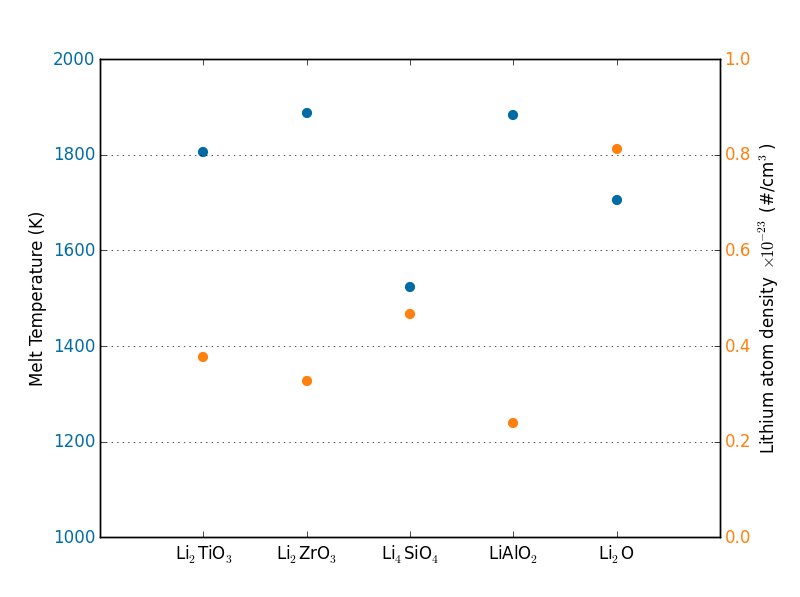
\includegraphics[width=0.75\textwidth]{images/tmelt-li-density} 
	\caption{Comparisons of melt temperature and lithium density for several lithium oxides.}
	\label{fig:tmelt-li-density}
\end{figure}

Performance of a reactor, however, will be strongly affected by its thermal conductivity and sintering characteristics. General material sintering temperature is generally considered as $0.8T_\text{melt}$ and all the materials shown in \Cref{fig:tmelt-li-density} show acceptable melt temperatures. However, neutron radiation typically enhances sintering characteristics and lowers temperatures at which sintering is observed. Indications are that radiation is expected to reduce sintering temperatures to around $0.6T_\text{melt}$


\lit has acceptable Li density, not hygroscopic, has lower activation, similar T release to \liz. Mechanically stronger than \lis.

\lis has weak crush strength, acceptable Li density, stable (can't read my notes)


\subsection{Tritium Release}


\subsection{Lithium ceramics}



Tritium release, a function of grain size, microsctructure, open/closed porosity. The material integrity is a functino of pebble size distribution, sphericity, mechanical strength, chemical stability.









% Last note on lithium... The average abundance of lithium in the Earth's crust is approximately 65 parts per million by weight. The concentration of lithium in sea water is also about 0.17 g/m$^3$. Lithium reserves are estimated to be sufficient for the United States' electrical demand for more than 600 years.















\section{Neutron multiplication in solid breeder}
(n,2n) reactions are always endothermic and therefore always have threshold energies

(n,2n) help raise tritium breeding ratio and increase neutrons for energy multiplication

The two most prominently analyzed neutron multipliers for a fusion reactor are beryllium and lead. Beryllium has a very high nuclide density while also being very light, with a high melting temperature, and high thermal conductivity. However it undergoes a 2-$\alpha$ reaction that causes trapped helium to swell the material. There is also a rarely occurring reaction with beryllium that generates tritium; it is frequent enough to cause a concern with contamination.

\begin{align}
\mathrm{n} + ~^9_4\mathrm{Be} &\xrightarrow ~2\mathrm{n}+2\alpha + \mathrm{T} -1.57~\text{MeV}\label{eq:Be-n}
\end{align}

melting temperature of beryllium is \SI{1250}{\celsius}, melting temperature of lead is \SI{327}{\celsius}. Thermal energy of Be is 1.7 MeV, Pb is 7 MeV. Choose beryllium for non-mobile breeder.

Chemical composition of beryllium,
\begin{itemize}
\item{BeO}
\begin{itemize}
\item{excellent compatibility with structural steel}
\item{carciongen, causes beryllium disease if inhaled}
\end{itemize}
\item{Be}
\begin{itemize}
\item{incompatibility with strucuture steel, forming FeBe13}
\item{Be reaction with water forming BeO (Be + H2O -> BeO + H2)}
\item{2Be + O2 -> 2BeO}
\end{itemize}
\item{Be12Ti}
\begin{itemize}
\item{compatible with ss.}
\item{high metling temperature}
\item{less swelling than Be}
\item{higher chemical stability}
\item{high Be density maintains neutron multiplication characteristics}
\end{itemize}
\end{itemize}
Bear in mind limited Be abundancy on Earth. (remember Homework set)

Beryllium will also exist as a pebble bed. The following reaction has small probability of occurrence (check cross-section for this reaction)
\begin{align}
\mathrm{n} + ~^9_4\mathrm{Be} &\xrightarrow ~ ^4_2\mathrm{He} +~^6_2\mathrm{He}\\
~^6_2\mathrm{He} &\xrightarrow ~ ^6_3\mathrm{Li} + \beta^-\\
\mathrm{n} + ~^6_3\mathrm{Li} &\xrightarrow ~ T + \alpha
\end{align}

Diffusional release of T from irradiated beryllium is very slow, measured in BeO to be about \num{1e-15} cm2/sec at 900C. The diffusional path should be kept aroudn 1 micron for T inventory concerns.























Disadvantages of lithium
\begin{itemize}
\item {It is chemically active meaning safety is an issue. As an example, here are two reactions with oxygen along with their heats of formation
\begin{align*}
2\mathrm{Li} + \frac{1}{2}\mathrm{O} &\rightarrow \mathrm{Li}_2\mathrm{O} - 142.75~\text{kCal/mol}\\
2\mathrm{Li} + \mathrm{O} &\rightarrow \mathrm{Li}_2\mathrm{O}_2 - 151.9~\text{kCal/mol}
\end{align*}
note: a negative heat of formation means an exothermic reaction. Lithium will exothermically react with water (or air, concrete, or any moisture-containing materials) with high amounts of energy released. Of primary concern in lithium fires is the peak flame temperature. This will determine, to a large extent, whether many radioactive species become air-borne by vaporization. The flame temperature depends on many variables. Some investigations found it to be  about 2500 K which would cause some materials to melt but not vaporize.}
\item MHD effects -- liquid metals have high electrical conductivity. In a magnetic field this leads to a $\vec{J}\times\vec{B}$ force. This in turn leads to pressure drops in the magnetic fluid. To overcome the pressure drop requires increased pressurization and pumping power. The increase in pressurization leads to an increase in stresses of the containing structures and pumping power means more leeching of power from the reactor power plant.
\item Liquid metals tend to be corrosive. Corrosion products transport from radioactive structural materials and are carried downstream into sensitive regions.
\end{itemize}















Pebble form chosen for open porosity, large surface area to volume, maintain wall contact. But note that pebble bed is not the only solution. It is a good choice to satisfy the design requirements but pebble beds make a low conductivity material even worse at thermal transport.

Nevertheless, focusing on pebble bed form... specific performance requirements...



\section{Introduction to Solid Breeder Designs}
Common features of pebble bed designs...

low pressure, slow mass flow rate helium purge gas to extract T. High pressure coolant in structure. Permissible temperature window of Li bed. All heat removal via conduction to walls (through contacts and helium).

\subsection{Purge gas}
Purge - keep delta-P around 0.01 MPa. mdot = 0.1 to 0.3 g/s.

Review pressure drop correlations.

\subsection{Coolant}

Example values: coolant - P = 8 MPa. Tin = 300 C, Tout = 500 C (kept below 600 C for structural integrity of container).

Nothing exotic. standard heat transfer of a fluid in a duct. Must consider safety issues of high pressure coolant.

\subsection{Pebble bed}
(Discuss how its treated as a continuum, etc.)



\begin{enumerate}
\item{Always separately cooled with (with \textit{e.g.} helium or water)}
\item{Necessity of neutron multiplication}
\item{Surrounded by a structure of reduced-activation ferritic steel}
\end{enumerate}



A solid, non-mobile tritium breeding concept was first introduced by Abdoul\cite{Abdou1975} in 1975. The solid breeder concept satisfies the requirements of a breeder unit: transmute lithium into tritium, act as shield to other sensitive equipment and personnel, and convert energy into extractable heat for electricity production. Reference solid breeder designs have converged toward helium-cooled pebble beds (HCPB) of lithium ceramics.  The HCPB design incorporates packed beds of ceramic pebbles (spherical particles) that are filled into containment structures of a reduced-activation steel. In a typical solid breeder module, the breeding volume is subdivided into several alternating layers of neutron multiplication material (generally beryllium) and tritium breeding material. The layers are separated by plates with internal channels for coolant. Coolant is typically a high pressure helium, though some designs call for pressurized water, in spite of the dangers of the highly exothermic reaction of lithium with oxygen from water vapor in the case of coolant leak. The coolant, heated as it passes through the tritium breeding module, proceeds into a standard electricity production cycle. After tritium is generated inside the ceramic, the bred hydrogen isotope diffuses through the bulk material until being picked up by a low-pressure, slow moving purge gas (primarily helium) and extracted in a closed loop for fuel. Pebble bed forms of tritium breeding volumes have several advantages which include: ease of assembly of granular materials into complex geometries; bred tritium can be readily removed \textit{via} a helium purge gas through interstitial porous networks; ceramic material is unaffected by the large magnetic fields confining the plasma, and temperature gradients across any single pebble are small enough to avoid damage from thermal stress. A sketch of a generic volume of ceramic pebble bed is given in \Cref{fig:solid-breeder-sketch}

\begin{figure}[ht]
	\centering
	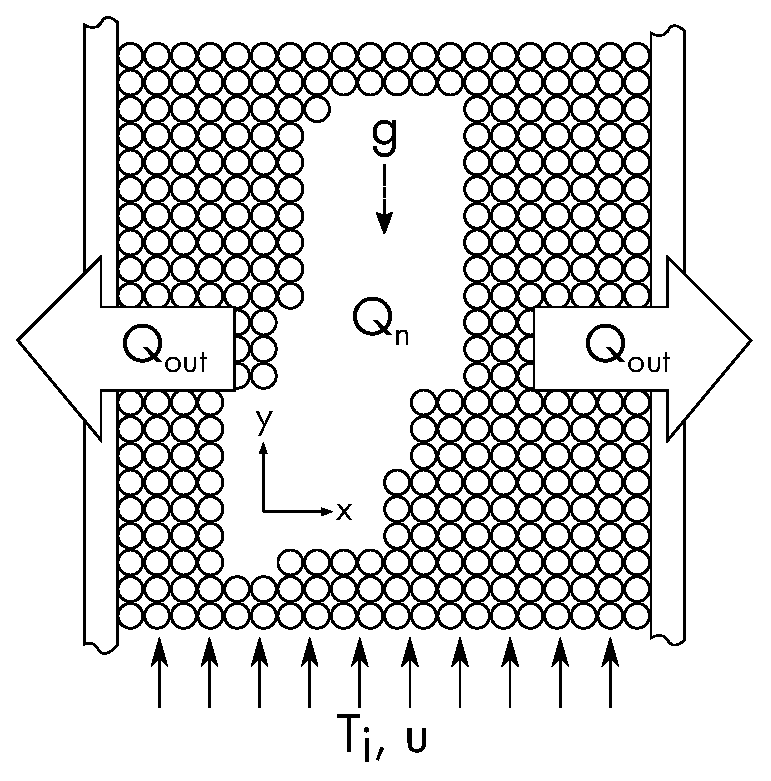
\includegraphics[width=0.6\textwidth]{images/x-domain} 
	\caption{Sketch of a typical unit of a pebble bed tritium breeding zone. The pebble bed is cooled with contact to the containing structure.}
	\label{fig:solid-breeder-sketch}
\end{figure}

A relatively narrow operational temperature window for optimum breeding performance of ceramics must be observed to respect temperature-dependent phenomena driving tritium release from lithiated ceramic pebbles, as will be discussed in detail in the following section. It is therefore necessary to have accurate knowledge of ceramic pebble bed thermomechanical behavior and comprehensive characterization; reliable models of heat transfer in solid breeders are critical for solid breeder designs. However, temperature prediction in ceramic pebble beds remains a challenge for many reasons. After packing the ceramic pebbles into a containment structure, there exists a coupling between mechanical forces acting upon beds and their heat transport capabilities. In addition, some amount of restructuring of the pebble bed and the internal contact force network is likely to occur in HCPBs from crushing/cracking of individual pebbles, inter-pebble sintering, or creep during operation. Contact conduction in beds, intimately linked to the packing structure, will subsequently be impacted during operation of ceramic pebble beds in fusion reactors. Concurrently, interaction of the slow-moving purge gas with tightly packed pebble beds is an additional route of heat transfer that must be understood. Thus, heat transfer in pebble beds is quite different from standard solid materials and requires specialized modeling of the synergistic physics. Knowledge and characterization of thermal transport must anticipate changes to the heat transfer capabilities and predict temperature profiles for pebble bed packing structures that will emerge after initially-packed pebble beds react to prolonged exposure to fusion reactor environments.

\section{Solid Breeder Thermal Management and Imposed Temperature Window}

To understand the importance of predictive capabilities of temperature in solid breeders, we first consider that one of the main roles of the breeder is to allow tritium to be readily extracted. Thus we need to understand tritium's journey from generation until it is swept away in helium purge gas. The process is shown schematically in \Cref{fig:mechanisms_tritium_transport}. Tritium begins its life internally inside a pebble's bulk. Tritium then diffuses most-slowly through the ceramic lattice until reaching a grain boundary. Along grain boundaries tritium diffuses more quickly and proceeds until reaching a surface of open porosity where it may desorb into the stagnant gas in a pebble's open porosity. Finally, tritium diffuses more rapidly still through the gas until being swept up in the advection of helium purge gas.\cite{Federici1990} 

\begin{figure}[ht]
    \centering
    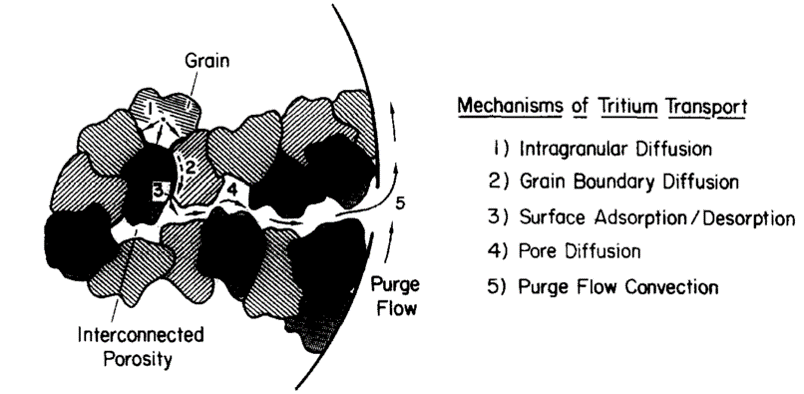
\includegraphics[width=0.6\textwidth]{images/mechanisms_tritium_transport} 
    \caption{Mechanisms of tritium transport in a single pebble\cite{Federici1990}.}
    \label{fig:mechanisms_tritium_transport}
\end{figure}

Experiments on tritium inventory have attempted to quantify the speeds of tritium release and found that bulk diffusion of tritium, typically the slowest transport mode, is a direct function of temperature.\cite{Franza2013} Thus the lower temperature limit, $T_\text{min}$, of temperature windows for solid breeders, is based on the unacceptable tritium inventory due to slow bulk diffusion. The value of $T_\text{min}$ is generally around \SI{300}{\celsius}. Using the same model of tritium transport, bulk diffusion also limits the maximum temperature in the solid breeder temperature window. At the other end of temperature spectrum, exposure to prolonged high temperature environments causes individual grains in a pebble to grow. Grain growth therefore extends the characteristic length of the slowest mode of tritium transport. Consequently, the maximum temperature, $T_\text{max}$, of the operational window for ceramic pebble beds is generally placed around 80\% of the melt temperature of the ceramic, $T_\text{max} = 0.8 T_\text{melt}$, to avoid surface sintering. For many lithium ceramics, this value falls around \SI{900}{\celsius}.

As a consequence of the tritium release from the solid breeder material, we are faced with a relatively narrow operational temperature to which solid breeder designers must adhere. Thus to provide designers the ability to optimize breeder volumes for tritium breeding and subsequent tritium release, we must understand the important physics and phenomena dictating thermomechanical responses of pebble beds during operation in a fusion reactor.




% High energy (14 MeV) neutrons are ejected from the deuterium-tritium reaction, as described by \Cref{eq:dt-reaction}
% \begin{align}
%     \mathrm{D} + \mathrm{T}&\xrightarrow{}\ ^4\mathrm{He}+\mathrm{n}+17.58\ \text{MeV} \label{eq:dt-reaction}
% \end{align}
% thus t

Tritium breeding blankets will experience high volumetric heating as deposited by high-energy neutrons that are carrying away approximately 80\% of the fusion reaction energy as well as secondary $\gamma$ rays. The deposited heat must be transported through the pebble bed region into the walls of the containing structure, then ultimately into the coolant gas. Heat deposited into pebble beds will transfer \textit{via} inter-particle contact conduction, inter-particle radiation, and convection with the helium purge gas. At the interface with the structural material, similar modes of heat transfer are present: particle-wall contact conduction, particle-wall radiation, and communication \textit{via} helium purge gas convection. As the pebbles heat under the nuclear load, thermal expansion of the pebbles in the packed volume will be contained by cooler structural material. Confined expansion will give rise to increased contact pressure between pebbles. Pressure on pebble beds is known to be the cause of many phenomena, some of which directly impact the thermal transport characteristics of pebble beds and may ultimately jeopardize the reliable and safe operation of breeding blankets. 

The packing structure of packed beds can be considered as a metastable configuration that will last indefinitely unless acted upon by an external perturbation such as vibration or compressive pressure.\cite{Jaeger1996} The ability of a metastable configuration to resist perturbations can in some way be quantified by the initial packing fraction. For more compliant beds, with lower packing fractions, stresses from thermal expansion can cause significant rearrangement of the packing structure which is not recoverable after stress removal. This phenomena has been observed in numerous experiments as so-called plastic rearrangement of pebble beds.\cite{Reimann:2002kl,Reimann:2000tw,Zhang2015} Plasticity of beds may have significant consequences for the ability of the pebble bed to maintain contact with the containing structure and routes for heat out of the bed due to gap formation between pebble volumes and coolant walls. Moreover, increased pressure between pebbles can cause the brittle pebbles themselves to fragment which will also disrupt paths of heat in the inter-particle conduction network. The consequence of both aformentioned effects is an increase in the temperature of bed pebbles. If the fragments are sufficiently small, they may even cause blockage of the helium purge gas. 

Due to the complicated nature of granular materials such as ceramic pebble beds, heat transfer in these solid breeder volumes should not be considered as a static phenomena that can be characterized prior to inserting pebbles beds into breeder modules and then expected to behave consistently after long exposure to fusion environments. Pebble bed temperatures, linked to the packing, will evolve in ways that are currently not predictable and must be studied and modeled.

In spite of their many engineering applications, heat transfer mechanisms in packed beds of granular material are still not thoroughly understood nor characterized. Hence, one approach is to treat the granular material as a fictitious continuous media, an approach adopted by several designers of solid breeders. Many experiments have been carried out for developing phenomenological models for effective material properties. In this approach, heat transport in pebble beds is often characterized with an effective thermal conductivity, $k_\text{eff}$, and interface heat conductance. Many models have shown their ability to accurately predict the temperature profiles for pebble beds under specific operating conditions. However, the accuracy of the model predictions often degrade as soon as a pebble bed's granular material, grain radii distributions, or operating conditions vary from the experimentally studied packed beds. In addition, propensity for creep, crushing, and inter-particle sintering of ceramic materials alter the packing structure in ways not currently predictable with the effective material characterizations. Furthermore, effective conductivity models that consider interstitial gas often assume the gas is stagnant. The assumption has not been thoroughly vetted and is likely insufficient to capture the thermal influence of the helium purge gas flowing through the ceramic pebble beds in fusion reactors.

To overcome the limitations of effective material modeling, and aided by the acceleration and availability of computational power, many researchers of granular heat transfer have shifted their attention to studies of the interacting physics on pebble-scales. In this approach, we interrogate heat transfer on the scale of contact conductance between interacting particles and directly model transient behaviors of packed beds. We can then couple particle-scale models of heat transfer and mechanics to either volume-averaged fluid models or models of the entire tortuous fluid flow through the porous network of packed beds.






\chapter{Solid Breeder Analysis}

\section{Pressure drop}
P.C. Carman\cite{Carman1997}, using Kozeny's Equation as a starting point, derived a formula for pressure drop per length of a packed bed at the close-packed limit,
\begin{equation}\label{eq:K-C-pressure}
    \frac{\Delta p}{L} = \frac{180 \bar{U} \mu}{d_p^2} \frac{(1-\epsilon)^2}{\epsilon^3}
\end{equation}
where $\mu$ is the viscosity, $\epsilon$ is the void fraction, $d_p$ is the particle diameter (assuming spherical) and $\bar{U}$ is the superficial velocity of the fluid in the packed bed.

Carman points out the limitations of applicability of the Kozeny-Carman (KC) equation: built into the equation is the assumption that the range of pore size and shape is fairly isotropic and similarly the tortuosity through the packed bed is relatively uniform. Pressure drop as a function of Reynolds number for \SI{1}{\milli\meter} particles in a packing fraction of $\phi = 1-\epsilon = 0.645$ in helium at \SI{600}{\celsius} is given in \Cref{fig:KC-pressure-drop}.

\begin{figure}[ht]
    \centering
    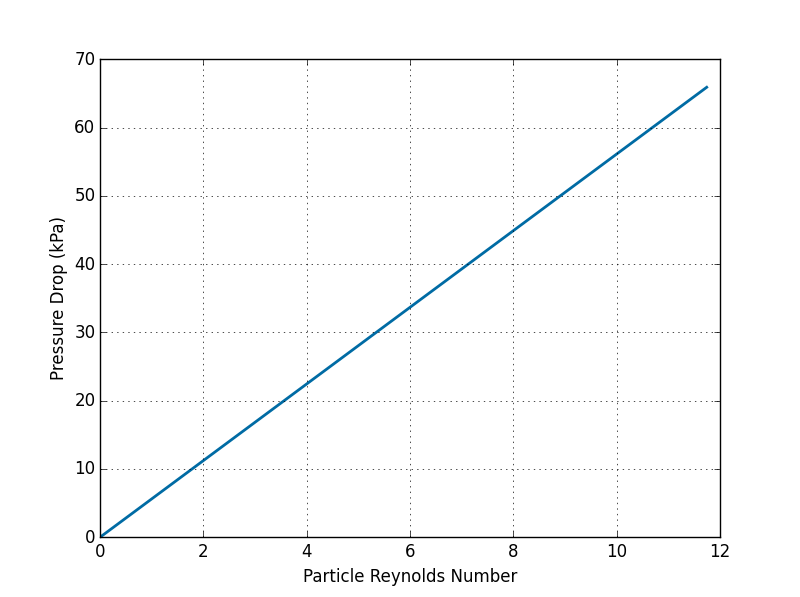
\includegraphics[width=\textwidth]{images/KC-pressure-drop}
    \caption{Kozen-Carman pressure drop increases linearly with particle Reynolds number.}
    \label{fig:KC-pressure-drop}
\end{figure}



\section{Effective conductivity}
Deissler and Boegli, in 1958, proposed upper and lower bounds of effective thermal conductivity, $k_\text{eff}$, in two-phase granular media to be given by alternating layers of the two phases arranged in parallel or series, respectively \cite{Deissler1958}. In the case of parallel layers, effective conductivity, normalized by fluid conductivity, is
\begin{equation}\label{eq:keff-parallel}
	\frac{k_e}{k_f} = \epsilon + (1-\epsilon)\kappa
\end{equation}
where $k_f$ is the fluid conductivity, $\kappa = k_s/k_f$ is the ratio of solid to fluid conductivity, and $\epsilon$ is the void fraction in the porous media. Similarly, the minimum effective conductivity is found in a serial layering of the solid and fluid phases,
\begin{equation}\label{eq:keff-series}
	\frac{k_e}{k_f} = \frac{1}{\epsilon + (1-\epsilon)/\kappa}
\end{equation}
\Cref{eq:keff-parallel,eq:keff-series} act as theoretical upper and lower limits to true effective thermal conductivities of real material.

One of the most widely-used correlations was put forth by Zehner and Schlunder in 1970 \cite{Zehner1970,Zehner1972}. They considered a cylindrically-shaped unit cell and made the analogy between heat and mass transfer to derive an empirical fit to data in the bulk of two-phase porous media. The Zehner-Schlunder (ZS) correlation is
\begin{equation}
    \frac{k_e}{k_f} = \left(1-\sqrt{1-\epsilon}\right)+\frac{2\sqrt{1-\epsilon}}{1-B/\kappa}\left[\frac{(1-1/\kappa)B}{(1-B/\kappa)^2}\ln\left( \frac{\kappa}{B} \right) - \frac{B+1}{2} - \frac{B-1}{1-B/\kappa}\right]
\end{equation}
where $B$ is a deformation parameter related to porosity as
\begin{equation}\label{eq:zs-B}
    B = 1.25\left(\frac{1-\epsilon}{\epsilon}\right)^{1.11}
\end{equation}

\begin{figure}[ht]
    \centering
    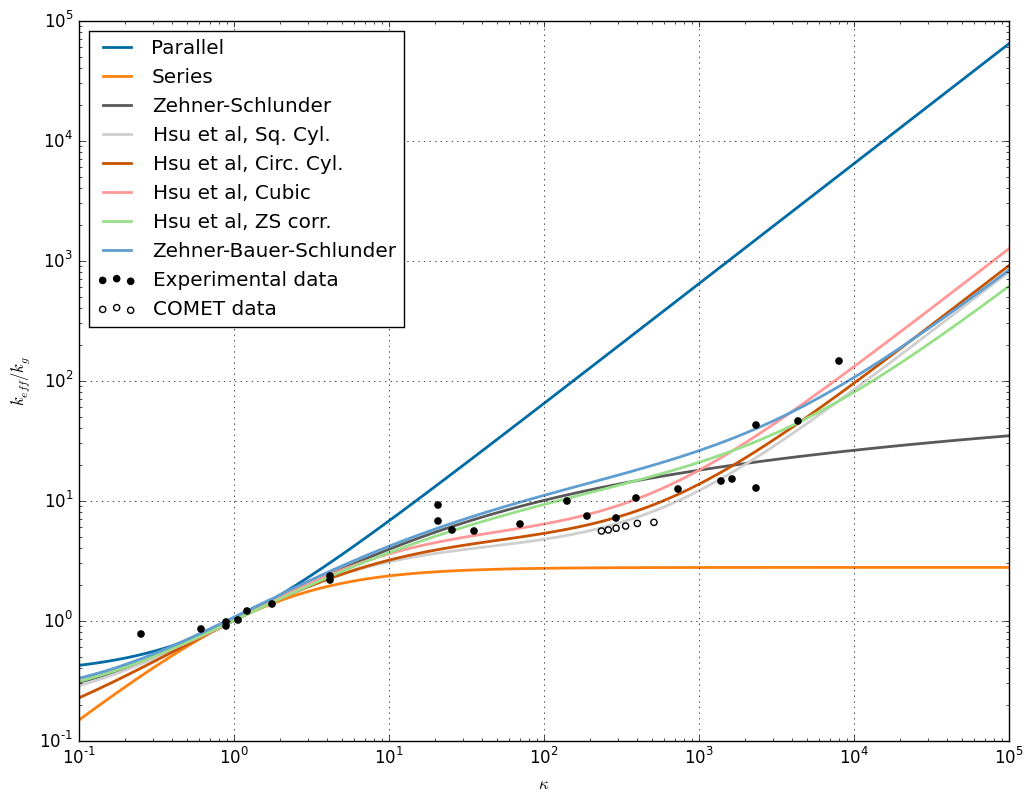
\includegraphics[width=\textwidth]{images/keff-kappa-experimental-comet}
    \caption{Comparison of COMET data on IG11 graphite, $k_\text{eff}$ correlations, and experimental data. Data compiled by \cite{VanAntwerpen2010} from many sources and measured data at UCLA.}
    \label{fig:kappa-experimental-comet}
\end{figure}


\end{document}